% Filename: slide01.tex
% This code is part of 'Cursos CAMECC: Introducao ao LaTeX para o Curso 29 - Licenciatura em Matematica'
% 
% Description: This file correspond to the slides of using for cap01@camecc_lic.tex of the course.
% 
% Created: 07.06.12 11:30:10 AM
% Last Change: 07.06.12 11:30:30 AM
% 
% Authors:
% - Raniere Silva, r.gaia.cs@gmail.com
% 
% Organization: CAMECC - Centro Academico dos Estudantes do IMECC
% 
% Copyright (c) 2012, Raniere Silva. All rights reserved.
% 
% This work is licensed under the Creative Commons Attribution-ShareAlike 3.0 Unported License. To view a copy of this license, visit http://creativecommons.org/licenses/by-sa/3.0/ or send a letter to Creative Commons, 444 Castro Street, Suite 900, Mountain View, California, 94041, USA.
%
% This work is distributed in the hope that it will be useful, but WITHOUT ANY WARRANTY; without even the implied warranty of MERCHANTABILITY or FITNESS FOR A PARTICULAR PURPOSE.
%
\documentclass[12pt]{beamer}
\usetheme{CambridgeUS}
\let\Tiny=\tiny  % Redefine at least \Tiny for avoid warning
% Filename: use_pack.tex
% This code is part of 'Cursos CAMECC: Introducao ao LaTeX para o Curso 29 - Licenciatura em Matematica'
% 
% Description: This file is only a list of the packages used in the course.
% 
% Created: 07.06.12 11:30:10 AM
% Last Change: 07.06.12 11:30:30 AM
% 
% Authors:
% - Raniere Silva, r.gaia.cs@gmail.com
% 
% Organization: CAMECC - Centro Academico dos Estudantes do IMECC
% 
% Copyright (c) 2012, Raniere Silva. All rights reserved.
% 
% This work is licensed under the Creative Commons Attribution-ShareAlike 3.0 Unported License. To view a copy of this license, visit http://creativecommons.org/licenses/by-sa/3.0/ or send a letter to Creative Commons, 444 Castro Street, Suite 900, Mountain View, California, 94041, USA.
%
% This work is distributed in the hope that it will be useful, but WITHOUT ANY WARRANTY; without even the implied warranty of MERCHANTABILITY or FITNESS FOR A PARTICULAR PURPOSE.
%
\usepackage[brazil]{babel}
\usepackage[utf8]{inputenc}
\usepackage[T1]{fontenc} 
\usepackage{pb-diagram}
\usepackage{graphicx, color}
% \usepackage[top=3cm,left=2cm,right=2cm,bottom=3cm]{geometry} % Must be repeat in the file.
\usepackage{subfig}
\usepackage{enumerate}
\usepackage{algorithmic}
\usepackage{algorithm}
\usepackage{listings}
\usepackage{listingsutf8}
\usepackage{indentfirst}
\usepackage{multirow}
\usepackage{amsthm}
\usepackage{amsmath}
\usepackage{amsfonts}
\usepackage{amssymb}
\usepackage{makeidx}  % For index.
\makeindex  % For index.
\usepackage{tikz}
\usetikzlibrary{patterns}
\usepackage{epsfig}
\usepackage{latexsym}
\usepackage{makeidx}
\usepackage{url}
\usepackage{hyperref}
\usepackage{breakurl}
\usepackage{multicol}
\usepackage{parcolumns}
\usepackage[official]{eurosym}
\lstset{
breaklines=true,
literate={é}{{\'e}}1 {á}{{\'a}}1 {ã}{{\~a}}1,
}

\renewcommand{\lstlistingname}{Código}
\lstset{
language=TeX,                   % the language of the code
basicstyle=\ttfamily\footnotesize,     % the size of the fonts that are used for the code
%numbers=left,                   % where to put the line-numbers
%numberstyle=\footnotesize,      % the size of the fonts that are used for the line-numbers
%stepnumber=5,                   % the step between two line-numbers. If it's 1, each line 
%numbersep=5pt,                  % how far the line-numbers are from the code
showspaces=false,               % show spaces adding particular underscores
showstringspaces=false,         % underline spaces within strings
showtabs=false,                 % show tabs within strings adding particular underscores
tabsize=2,                      % sets default tabsize to 2 spaces
%captionpos=t,                   % sets the caption-position to bottom
breaklines=true,                % sets automatic line breaking
breakatwhitespace=false,        % sets if automatic breaks should only happen at whitespace
%caption={\texttt{\lstname}},    % show the filename of files included with \lstinputlisting;
}

% New commands and enviromments
\newcommand{\TikZ}{Ti\emph{k}Z }
\newcommand{\PGF}{\textsc{PGF} }
\newcommand{\lcode}[1]{\texttt{#1}}  % Code in the same line.
\lstnewenvironment{code}{}{}  % Code in new line.
\newcommand{\fcode}[1]{\lstinputlisting[firstline=18]{#1}}  % Code in a file.
\newcommand{\example}[1]{  % For examples.
\begin{minipage}[htb]{0.55\textwidth}
    \fcode{#1}
\end{minipage} \hfill \vrule \hfill
\begin{minipage}[htb]{0.35\textwidth}
    \include{#1}
\end{minipage}
}


\begin{document}
\title[Introdu\c{c}\~{a}o ao LaTeX - 01/04]{Cursos CAMECC \\ Introdu\c{c}\~{a}o ao LaTeX para o Curso 29 \\ Licenciatura em Matem\'{a}tica \\ Aula 01}
\author{Raniere Silva}
\institute[CAMECC]{Centro Acad\^{e}mico dos Estudantes do IMECC}
\begin{frame}
    \titlepage
\end{frame}

\begin{frame}
    \frametitle{Licen\c{c}a}
    Este trabalho foi licenciado com a Licen\c{c}a Creative Commons Atribui\c{c}\~{a}o - CompartilhaIgual 3.0 N\~{a}o Adaptada. Para ver uma c\'{o}pia desta licen\c{c}a, visite \url{http://creativecommons.org/licenses/by-sa/3.0/} ou envie um pedido por carta para Creative Commons, 444 Castro Street, Suite 900, Mountain View, California, 94041, USA.
    %
    %Com base na obra dispon\'{i}vel em \url{https://github.com/r-gaia-cs/latex_with_vim/}. 
    %
    %Podem estar dispon\'{i}veis permiss\~{o}es adicionais ao \^{a}mbito desta licen\c{c}a em \url{https://github.com/r-gaia-cs/latex_with_vim/}.
    %
    \begin{center}
        
\includegraphics[keepaspectratio=true]{../../figures/cc-by-sa.png}
    \end{center}
\end{frame}

\begin{frame}
    \frametitle{Sum\'{a}rio}
    \tableofcontents
\end{frame}

\section{Informa\c{c}\~{o}es}
\begin{frame}
    \frametitle{Sobre o curso}
    \begin{enumerate}
        \item Introdu\c{c}\~{a}o.
        \item Figuras e Tabelas.
        \item Express\~{o}es Matem\'{a}ticas.
        \item Desenhos e Apresenta\c{c}\~{o}es.
    \end{enumerate}
\end{frame}

\begin{frame}
    \frametitle{\flang{Learning Pyramid}}
    \begin{center}
        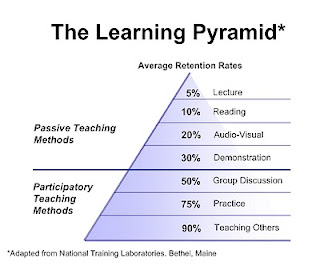
\includegraphics[height=0.6\textheight]{figures/learning_pyramid.jpg}
    \end{center}
    Imagem de Anna T. e dispon\'{i}vel em \url{http://3.bp.blogspot.com/_RC_EAn5VwgY/TS-tVyIU8yI/AAAAAAAAACU/o7szcDYN_FM/s1600/The-Learning-Pyramid.jpg}
\end{frame}
\begin{frame}
    \frametitle{Hist\'{o}ria}
    % Codificado de codes/history_timeline@latex_with_vim.tex
    \begin{tikzpicture}[xscale=0.15, yscale=0.4]
        \draw[gray!60] (46,0) grid (116,12);
        \foreach \y in {46, 56, ..., 96}{
            \node[below] at (\y, 0) {\y};
        }
        \node[below] at (106,0) {06};
        \node[below] at (116,0) {16};

        \draw[fill=red!60] (50,-1) rectangle ++(1,-1) ++(1,.5) node[right]{Hardware};
        \draw[fill=blue!60] (70,-1) rectangle ++(1,-1) ++(1,.5) node[right]{Sistema operacional};
        \draw[fill=green!60] (100,-1) rectangle ++(1,-1) ++(1,.5) node[right]{Software};

        \draw[fill=red!60] (46,0) rectangle (55,1) node[midway]{ENIAC};
        \draw[fill=blue!60] (69,1) rectangle (112,2) node[midway]{UNIX};
        \draw[fill=green!60] (83,2) rectangle (112,3) node[midway]{GNU Project};
        \draw[fill=blue!60] (91,3) rectangle (112,4) node[midway]{Linux Kernel};
        \draw[fill=green!60] (78,4) rectangle (112,5) node[midway]{\TeX};
        \draw[fill=green!60] (85,5) rectangle (112,6) node[midway]{\LaTeX};
        \draw[fill=red!60] (76,6) rectangle (78,7) node[midway]{Apple I};
        \draw[fill=red!60] (83,7) rectangle (85,8) node[midway]{Lisa};
        \draw[fill=blue!60] (84,8) rectangle (112,9) node[midway]{Mac OS};
        \draw[fill=blue!60] (81,9) rectangle (85,10) node[midway]{DOS};
        \draw[fill=blue!60] (85,9) rectangle (112,10) node[midway]{Windows};
        \draw[fill=green!60] (85,10) rectangle (112,11) node[midway]{Word};
        \draw[fill=green!60] (84,11) rectangle (100,12) node[midway]{StarOffice};
        \draw[fill=green!60] (100,11) rectangle (112,12) node[midway]{OpenOffice};
    \end{tikzpicture}
\end{frame}

\begin{frame}[fragile]
    \frametitle{Nomenclatura (1)}
    Comandos s\~{a}o da forma
    \begin{code}
\nome[opcoes]{parametro1}{parametro2}{...}
    \end{code}
    e alguns exemplos s\~{a}o \lstinline!\documentclass!, \lstinline!\usepackage! e \ldots
\end{frame}

\begin{frame}[fragile]
    \frametitle{Nomenclatura (2)}
    Ambientes s\~{a}o da forma
    \begin{code}
\begin{nome}[opcoes]
    parametro
\end{nome}
    \end{code}
    e alguns exemplos s\~{a}o \envname{document}, \envname{table}, e \ldots
\end{frame}

\begin{frame}
    \frametitle{TeXworks}
    \begin{center}
        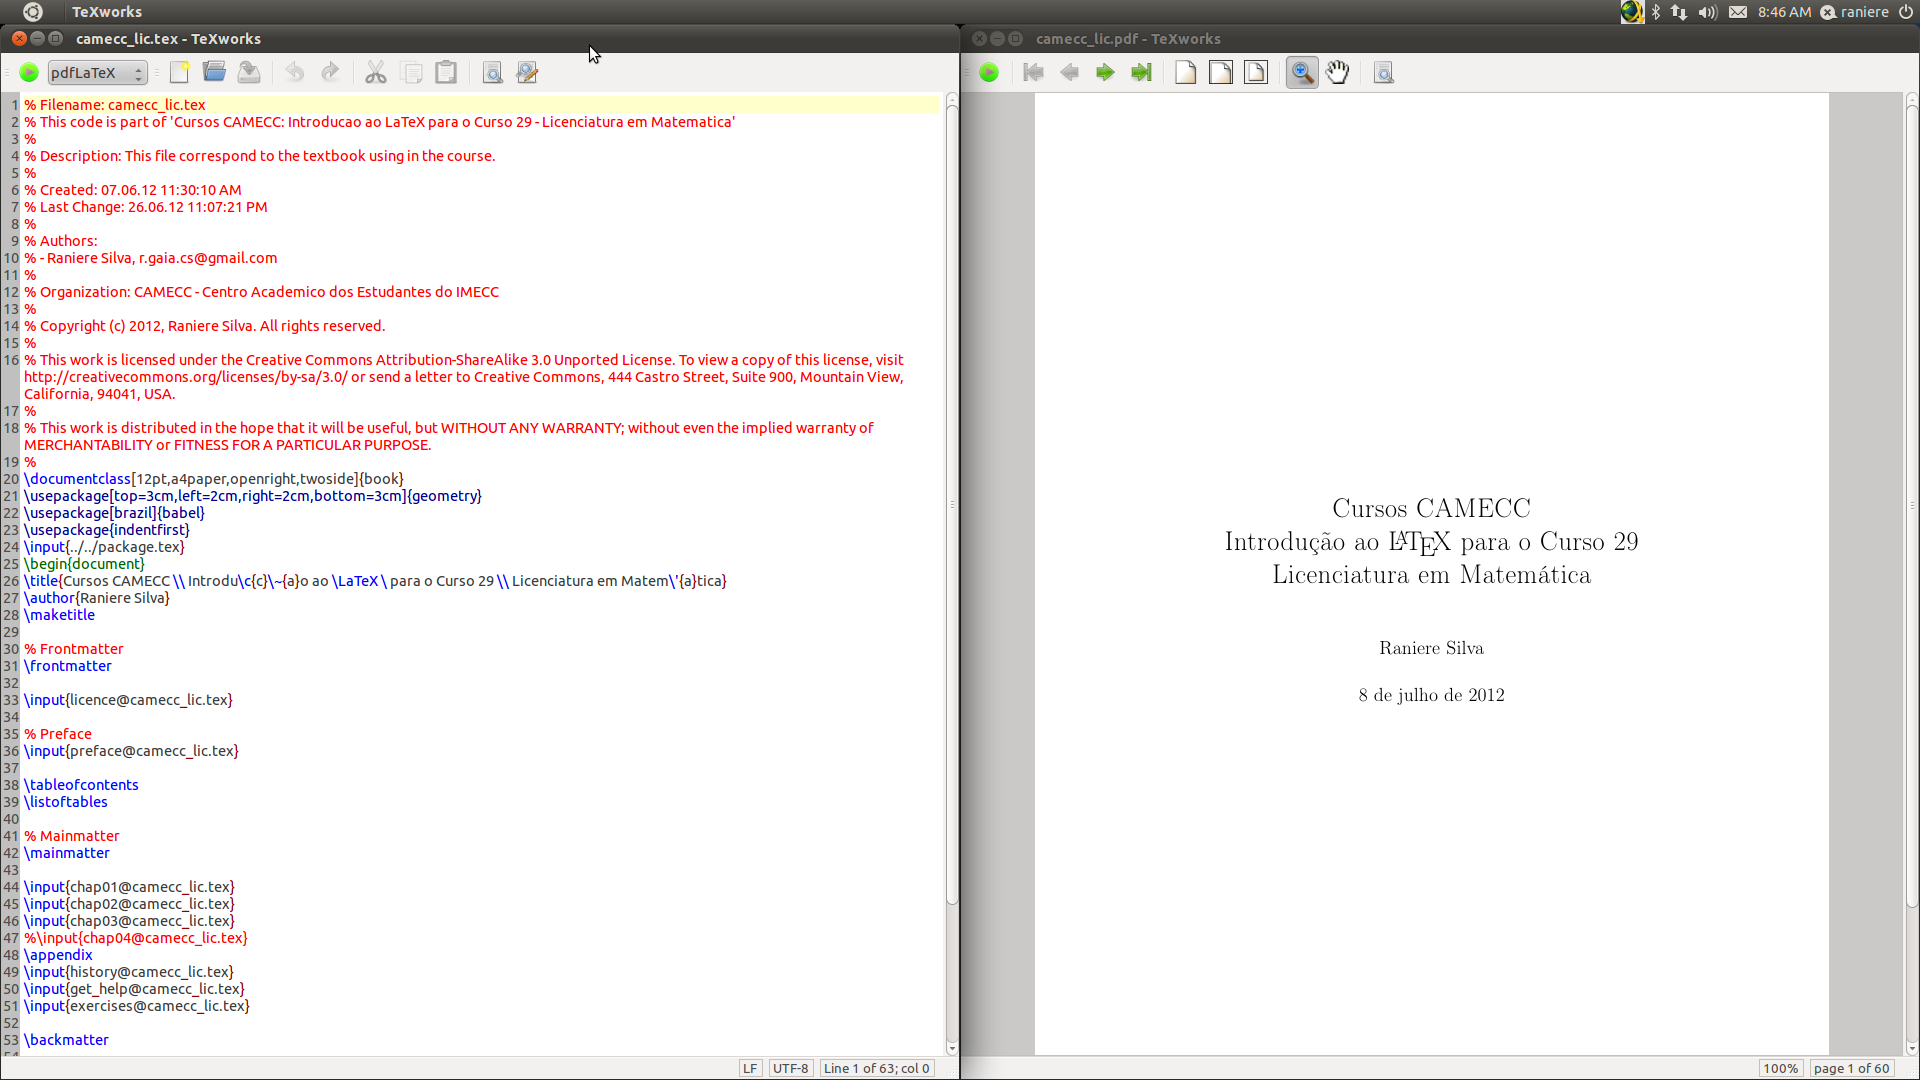
\includegraphics[width=0.8\textwidth]{figures/texworks.png}
    \end{center}
\end{frame}

\section{Hello world}
\begin{frame}[fragile]
    \frametitle{Hello world}
    \begin{code}
\documentclass[10pt,a4paper]{article}
\begin{document}
Hello world.
\end{document}
    \end{code}
\end{frame}

\begin{frame}[fragile]
    \frametitle{Hello world}
    \begin{code}
\documentclass[10pt,a4paper]{article}
\usepackage[utf8]{inputenc}
\begin{document}
Hello world.
\end{document}
    \end{code}
\end{frame}

\begin{frame}[fragile]
    \frametitle{Hello world}
    \begin{code}
\documentclass[10pt,a4paper]{article}
\usepackage[utf8]{inputenc}
\usepackage[T1]{fontenc} 
\begin{document}
Hello world.
\end{document}
    \end{code}
\end{frame}

\begin{frame}[fragile]
    \frametitle{Hello world}
    \begin{code}
\documentclass[10pt,a4paper]{article}
\usepackage[utf8]{inputenc}
\usepackage[T1]{fontenc} 
\begin{document}
Hello world.      Hello world.

Hello world. [2]
\end{document}
    \end{code}
\end{frame}

\begin{frame}[fragile]
    \frametitle{Hello world}
    \begin{code}
\documentclass[10pt,a4paper]{article}
\usepackage[utf8]{inputenc}
\usepackage[T1]{fontenc} 
\begin{document}
``Hello world.'' \ldots
\end{document}
    \end{code}
\end{frame}

\section{Formata\c{c}\~{a}o}
\begin{frame}[fragile]
    \frametitle{Hello world}
    \begin{code}
\documentclass[10pt,a4paper]{article}
\usepackage[utf8]{inputenc}
\usepackage[T1]{fontenc} 
\begin{document}
\textit{Hello world}.

\begin{LARGE}
    Hello world.
\end{LARGE}

\begin{center}
    Hello world.
\end{center}
\end{document}
    \end{code}
\end{frame}

\begin{frame}
    \frametitle{Fim}
    \begin{center}
        Perguntas.
    \end{center}
\end{frame}
\end{document}
